\documentclass{standalone}
\usepackage{pgfplots}
\begin{document}
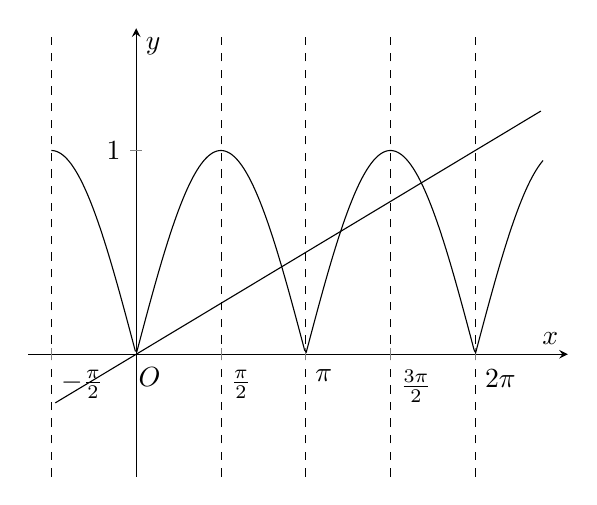
\begin{tikzpicture}
\begin{axis}
[
ymin=-0.6,ymax=1.6,
xmin=-2,xmax=8,
xtick=\empty,
ytick=\empty,
extra x ticks={-1.5708, 1.5708, 3.14159, 4.71239, 6.28319},
extra x tick labels={$-\frac{\pi}{2}$, $\frac{\pi}{2}$, $\pi$, $\frac{3\pi}{2}$, $2\pi$},
extra y ticks={1},
extra y tick labels={$1$},
every extra x tick/.style={
    xticklabel style={anchor=north west},
    grid=major,
    major grid style={very thin,dashed,black}
},
axis lines = center,
xlabel=$x$,ylabel=$y$,
samples=200,
]
\addplot [black, domain=-1.5708:7.53982, samples=300] {abs(sin(deg(x)))};
\addplot [black, domain=-1.5:7.5] {x/(2*pi)};
\node at (axis cs:0.25, -0.11) {$O$} ;
\end{axis}
\end{tikzpicture}
\end{document}
